% Main LaTeX file for the thesis/project report
\documentclass[12pt,a4paper]{report}

% Encoding and language
\usepackage[utf8]{inputenc}
\usepackage[T1]{fontenc}
% Times text + math fallback
\usepackage{mathptmx} % Times New Roman-like; body 12pt via class option
\usepackage[english]{babel}

% Page and typography
\usepackage{geometry}
\geometry{margin=1in}
\usepackage{setspace}
\onehalfspacing
% Paragraph formatting: no indent, no extra spacing; keep full justification
\setlength{\parindent}{0pt}
\setlength{\parskip}{0pt}
% Heading sizes per requirement
\usepackage{titlesec}
% Number all levels for TOC (chapters, sections, subsections, subsubsections),
% but only print numbers on sections in the body.
\setcounter{secnumdepth}{3}
\setcounter{tocdepth}{3}
% Apply sizes to heading text; no printed numbers
\titleformat{\chapter}[display]{\bfseries\centering\fontsize{16pt}{18pt}\selectfont}{}{0pt}{}
\titleformat{\section}{\bfseries\fontsize{14pt}{16pt}\selectfont}{\thesection}{0.5em}{}
\titleformat{\subsection}{\bfseries\fontsize{14pt}{16pt}\selectfont}{\thesubsection}{0.5em}{}
\titleformat{\subsubsection}{\bfseries\fontsize{14pt}{16pt}\selectfont}{\thesubsubsection}{0.5em}{}
% Remove extra vertical gaps around headings; start at normal margins
\titlespacing*{\chapter}{0pt}{0pt}{12pt}
\titlespacing*{\section}{0pt}{6pt}{6pt}
\titlespacing*{\subsection}{0pt}{6pt}{6pt}
\titlespacing*{\subsubsection}{0pt}{6pt}{6pt}
\usepackage{microtype}

% Figures, tables, colors
\usepackage{graphicx}
\graphicspath{{../new_work/figures/}{../new_work/figures/new/}{../new_work/notebooks/}{../new_work/notebooks/new/}{../new_work/}}
\usepackage{caption}
\usepackage{subcaption}
\usepackage{booktabs}
\usepackage{multirow}
\usepackage{xcolor}
\usepackage{float} % For strict figure placement [H]

% Math
\usepackage{amsmath, amssymb, amsfonts}

% Hyperlinks
\usepackage[hidelinks]{hyperref}
\hypersetup{pdftitle={EfficientNetvs.CBAM}}
% Bibliography
\usepackage[numbers,sort&compress]{natbib}

% If available, allow including webp logos; otherwise fall back to png/pdf
% (README explains conversion if needed)
\newcommand{\unilogo}{project_report/logo/ru_logo}

% Title data
\newcommand{\reporttitle}{EfficientNet vs. CBAM: Benchmarking Attention for Ocular Disease Classification}
\newcommand{\supervisor}{Dr. Md. Matiqul Islam}
\newcommand{\authors}{Md. Takrim\textendash Ul\textendash Alam (Roll: 1911177149)\\ Samiul Bashir (Roll: 2010277105)}
\newcommand{\department}{Department of Information and Communication Engineering}
\newcommand{\university}{University of Rajshahi}
\newcommand{\reportdate}{\today}

\begin{document}

% Title page
\begin{titlepage}
  \centering
  % Try webp, then png, then pdf
  \IfFileExists{\unilogo.webp}{\includegraphics[width=0.25\textwidth]{\unilogo.webp}\\[1em]}{%
  \IfFileExists{\unilogo.png}{\includegraphics[width=0.25\textwidth]{\unilogo.png}\\[1em]}{%
  \IfFileExists{\unilogo.pdf}{\includegraphics[width=0.25\textwidth]{\unilogo.pdf}\\[1em]}{}}}
  {\LARGE \university\\[0.3em] \department\par}
  \vspace{2cm}
  {\huge\bfseries \reporttitle\par}
  \vspace{1.5cm}
  {\Large \textbf{Supervisor:} \supervisor\par}
  \vspace{0.8cm}
  {\Large \textbf{Authors:}\\ \authors\par}
  \vfill
  {\Large \reportdate\par}
\end{titlepage}

% Front matter
\clearpage
\pagenumbering{roman}

% Conditionally include Acknowledgement; omit when WITHOUTACK is defined
\ifdefined\WITHOUTACK
% (Acknowledgement omitted in this build)
\else
% Acknowledgements (moved to front, single page)
\chapter*{Acknowledgement}
At first, we would like to thank the Almighty Allah for giving us the opportunity to complete this project work successfully.

Foremost, we would like to thank our supervisor, Dr. Md. Matiqul Islam, Professor, Department of Information and Communication Engineering, University of Rajshahi, who continuously inspired and guided us during our project. We will forever be indebted to him for providing all the necessary help throughout the journey. He has not only supervised us but also provided advice, guidance, constant encouragement, and kind assistance. The thoughts he offered have enriched our project, without which this work would not have taken its present form.

Our parents have put us ahead of themselves. Because of their hard work and dedication, we have had opportunities beyond our wildest dreams. Our heartfelt thanks to them for giving us all we ever needed to be successful students and individuals.

Finally, we extend our gratitude to all the authors and researchers whose previous work on attention mechanisms, ocular disease analysis, and deep learning pipelines formed the foundation for this benchmarking between EfficientNet and EfficientNet+CBAM.
\fi

\clearpage
% Abstract page
\chapter*{Abstract}
\section*{Abstract}
This project investigates attention mechanisms for ocular disease classification using fundus images from the ODIR\textendash 5K dataset. We compare a strong convolutional baseline (EfficientNet) against an attention\textendash augmented variant employing the Convolutional Block Attention Module (CBAM). Our pipeline parses ODIR metadata, prioritizes Hypertension labeling where present, and enforces robust stratified splits to ensure all target classes appear in validation and test sets. Experiments demonstrate that image\textendash specific attention improves several classes, while Hypertension remains challenging due to limited single\textendash label prevalence and ambiguity in diagnosis text. We provide full training/evaluation artifacts (curves, confusion matrices, and metrics) to support reproducibility and future extensions, including multi\textendash label learning and targeted augmentation for rare classes.


\vspace{0.8em}
\textbf{Keywords:} EfficientNet, CBAM, ocular disease classification, ODIR\textendash 5K, Grad\textendash CAM, ROC\textendash AUC, PR\textendash AUC

\clearpage
% Front-matter order: TOC first, then LoF, then LoT
% Adjust TOC starting page based on whether Acknowledgement is included
\ifdefined\WITHOUTACK
\setcounter{page}{4} % roman iv when Acknowledgement is omitted
\else
\setcounter{page}{5} % roman v when Acknowledgement is present
\fi
\tableofcontents
\clearpage
\listoffigures
\clearpage
\listoftables
\clearpage

% Main matter
\pagenumbering{arabic}

% NOTE: The main topic names below should be aligned to the prior year's Table of Contents.
% Replace the section headings if your department requires exact titles.

% 1. Introduction (chapters start at normal margins, no extra vertical gaps)
\chapter{Introduction}
Retinal fundus photography provides a non\textendash invasive window into ocular health, enabling screening and diagnosis for conditions such as Glaucoma (G), Cataract (C), Age\textendash related Macular Degeneration (AMD, A), Hypertension\textendash related retinopathy (H), and Myopia (M). Automated classification can assist clinicians by prioritizing high\textendash risk cases and scaling screening programs.

Deep convolutional networks (CNNs) learn strong visual features but can struggle with class imbalance, domain variability, and subtle disease cues. Attention mechanisms explicitly reweight feature channels and spatial regions, potentially improving discrimination on small or ambiguous lesions. In this project we evaluate an EfficientNet baseline and an EfficientNet+CBAM variant on ODIR\textendash 5K, following a robust data parsing and splitting procedure, and report comprehensive metrics and plots to support a fair comparison.

\section{Contributions}
\begin{itemize}
  \item A practical ODIR\textendash 5K pipeline with robust parsing and Hypertension\textendash priority labeling to mitigate label sparsity in validation/test.
  \item An attention\textendash enhanced classifier (EfficientNet+CBAM) compared against a matched EfficientNet baseline under identical preprocessing, augmentation, and training schedules.
  \item Thorough evaluation artifacts (training curves, confusion matrices, ROC/PR curves, macro/weighted F1, ROC\textendash AUC and PR\textendash AUC) prepared for report integration.
\end{itemize}


% 2. Related Work
\chapter{Related Work}
\section{Fundus Image Classification}
CNNs such as VGG, ResNet, and EfficientNet have been widely applied to fundus image analysis for diabetic retinopathy screening and broader ocular disease classification. EfficientNet family models leverage compound scaling and strong ImageNet pretraining for competitive performance at modest compute cost \cite{tan2019efficientnet}.

\section{Attention Mechanisms}
Channel and spatial attention mechanisms (SE, CBAM, ECA) improve CNN feature quality by adaptively reweighting salient signals. CBAM applies sequential channel and spatial attention via lightweight modules with minimal overhead \cite{woo2018cbam}. For accessible primers on CBAM and related attention modules, see \cite{cbamMedium, cbamDO}. Vision transformers (ViT) and token\textendash based self\textendash attention have also shown promise, but often require larger datasets or heavy augmentation.

\section{ODIR\textendash 5K and Labeling}
The ODIR dataset provides paired left/right fundus images and metadata. Practical pipelines must reconcile free\textendash text diagnoses to structured labels and contend with multi\textendash label prevalence and class imbalance. Prior work also explored generative augmentation for minority classes.


% 2b. Expanded Literature Background
\chapter{Literature Review}
This review synthesizes clinical, architectural, and methodological evidence to ground our approach. We scoped sources to peer\textendash reviewed work and commonly cited practitioner guides, emphasizing fundus imaging practice and ocular disease foundations; CNN baselines and lightweight attention (SE, ECA, BAM, CBAM) alongside token\textendash based Transformers; and dataset/evaluation practices specific to ODIR\textendash 5K, including augmentation and explainability (Grad\textendash CAM, LIME/SHAP). Each strand maps directly to design: Hypertension\textendash aware labeling and patient\textendash level splits; an EfficientNet baseline with late CBAM placement for saliency control at low overhead; percent confusion matrices and macro metrics for imbalance; and Grad\textendash CAM validation that attention concentrates on clinically relevant regions. This integration underpins our hypothesis that CBAM improves separability and minority recall with modest parameter cost.

\section{Clinical and Modality Context}
A robust model must be grounded in the clinical realities and technical limitations of the data generation process. Fundus photography, while a standard diagnostic tool, is subject to numerous common pitfalls that can degrade dataset quality and, consequently, model reliability \cite{docxRef01,docxRef04,docxRef05}. These include artifacts such as camera\textendash lens dust, eyelash obstruction, poor patient fixation leading to blur, and improper illumination causing reflections or shadowed regions. Literature reviewing these practices \cite{docxRef04,docxRef05} informs the necessity of robust preprocessing and augmentation to ensure models are invariant to these non\textendash pathological variations. If not properly handled, a model might erroneously learn that an eyelash shadow is a sign of pathology, creating a ``shortcut'' feature that fails dramatically upon real\textendash world deployment.

Beyond modality artifacts, a firm clinical grounding is essential for defining class boundaries, especially given the high inter\textendash rater variability that can exist even among clinical experts. Our class definitions for Cataract and Age\textendash related Macular Degeneration (AMD) are informed by foundational literature \cite{docxRef07,docxRef08,docxRef09,docxRef12,docxRef13} that describes their expected image phenotypes. For cataracts, this primarily involves lens opacification obscuring the view of the retina, a feature the model must learn to identify. For AMD, this involves detecting key biomarkers in the macular region, such as drusen, pigmentary changes, or geographic atrophy \cite{docxRef09,docxRef12}.

Similarly, the diagnostic criteria for Hypertensive Retinopathy (H) are framed by clinical guidance \cite{docxRef14,docxRef15,docxRef16} focusing on vascular abnormalities. Our models must learn to capture subtle signs like arteriovenous (AV) nicking, copper or silver wiring of arterioles, flame\textendash shaped hemorrhages, and cotton\textendash wool spots, which are indicative of vascular damage from chronic hypertension. These signs can be subtle and often co\textendash exist with diabetic retinopathy, making a discriminative feature representation critical.

Finally, for the Myopia (M) class, we draw on references \cite{docxRef17,docxRef18} that contextualize the structural changes associated with high myopia and posterior staphyloma. These changes include significant globe elongation, which manifests in the fundus image as optic disc tilting, peripapillary atrophy, a tessellated fundus appearance, and lacquer cracks. This body of literature \cite{docxRef07,docxRef09,docxRef12,docxRef14,docxRef15,docxRef16,docxRef17,docxRef18} is critical for ensuring our model's feature extraction aligns with established clinical diagnostic criteria. This alignment is necessary to build a tool that is not just accurate, but also interpretable and trustworthy to a clinical end\textendash user.

\section{Architectures: CNNs, Transformers, and Attention}
The architectural design of a deep learning model is a primary determinant of its performance, balancing representational power with computational cost. CNNs have long been the \textit{de facto} standard in medical imaging \cite{docxRef19,docxRef20,docxRef21}, owing to strong inductive biases (spatial locality and translation invariance) that suit biomarker detection. We adopt EfficientNet \cite{tan2019efficientnet} as our CNN baseline for its state\textendash of\textendash the\textendash art accuracy\textendash efficiency trade\textendash off.

In contrast, Vision Transformers (ViT) \cite{dosovitskiy2021vit,docxRef23,docxRef24,docxRef25,docxRef26} adapt self\textendash attention to images by treating an image as a sequence of patches. ViTs offer a global receptive field and can model long\textendash range dependencies that may benefit diffuse ocular patterns. However, they often require massive pretraining and are computationally heavier than CNNs in low\textendash data settings typical of medicine.

Bridging these paradigms are attention modules that augment CNNs by helping them focus on salient signals. SE \cite{hu2018squeeze}, BAM \cite{park2018bam}, and CBAM \cite{woo2018cbam} are representative. We favor CBAM for its lightweight sequential design: first channel attention (\textit{what} to focus on), then spatial attention (\textit{where} to focus). This provides a compute\textendash efficient mechanism to refine EfficientNet features without sacrificing throughput, aiming for the best of both worlds: robust local feature extraction enhanced by attention\textendash driven selection.

\subsection{EfficientNet: Working Principle}
The core innovation of EfficientNet \cite{tan2019efficientnet} is compound scaling. Rather than scaling only one dimension (depth, width, or resolution), EfficientNet balances all three via a single coefficient \(\phi\): \(d=\alpha^{\phi}\), \(w=\beta^{\phi}\), \(r=\gamma^{\phi}\) under a compute budget. The MBConv inverted residual block forms the backbone: expand with a 1\texttimes1 conv, apply a depthwise separable conv for spatial mixing, then project with a 1\texttimes1 conv. Integrated SE attention \cite{hu2018squeeze} and Swish activations further improve efficiency and representational quality. This combination, paired with ImageNet pretraining, yields a strong, transfer\textendash effective baseline that we subsequently augment with CBAM.

\subsection{EfficientNet Architecture}
A practical overview of EfficientNet’s B0 design outlines a stem\textendash body\textendash head pipeline and details MBConv blocks with squeeze\textendash and\textendash excitation (SE), depthwise separable convolution, and swish activations \cite{tan2019efficientnet}. The B0 architecture starts with a 3\texttimes 3 stride\textendash 2 stem conv, proceeds through stages of MBConv with varying expansion ratios, kernel sizes (3\texttimes 3, 5\texttimes 5), and strides, and ends with a 1\texttimes 1 conv, global average pooling, and a fully connected classifier. This description matches our baseline configuration and motivates CBAM insertion on top of EfficientNet feature blocks.

\begin{figure}[H]
  \centering
  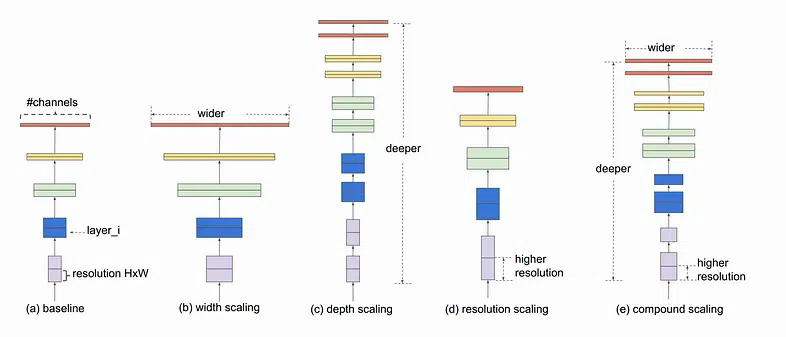
\includegraphics[width=0.92\textwidth]{../new_work/websites/Efficientnet Architecture - GeeksforGeeks_files/1_-ENqv4TI0JuyY6Nq8XQlAA.png}
  \caption{Scaling strategies summarized: individual width/depth/resolution scaling versus compound scaling that jointly balances all three.}
  \label{fig:effnet_gfg_scaling}
\end{figure}

\begin{figure}[H]
  \centering
  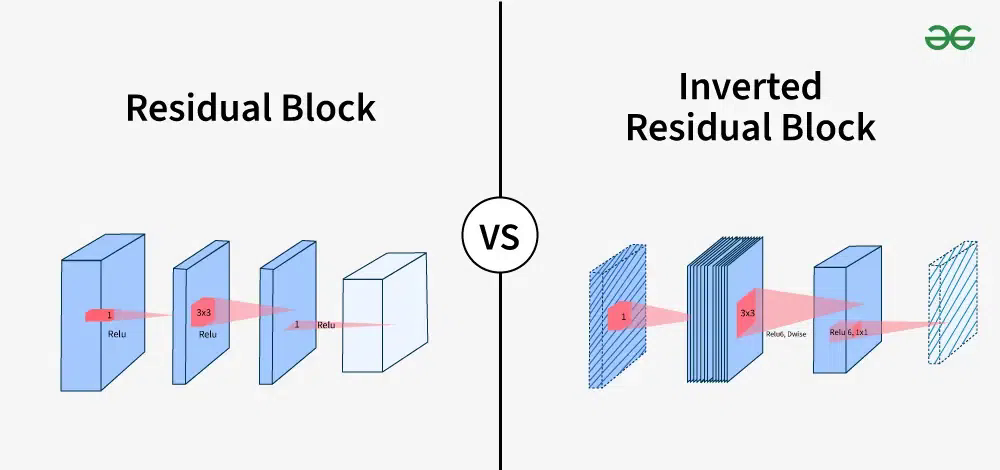
\includegraphics[width=0.92\textwidth]{../new_work/websites/Efficientnet Architecture - GeeksforGeeks_files/Residual-Block-vs-Inverted-Residual-Block.png}
  \caption{Residual vs inverted residual blocks illustrating EfficientNet’s MBConv design with depthwise separable conv and SE attention.}
  \label{fig:effnet_gfg_mbconv}
\end{figure}

\begin{figure}[H]
  \centering
  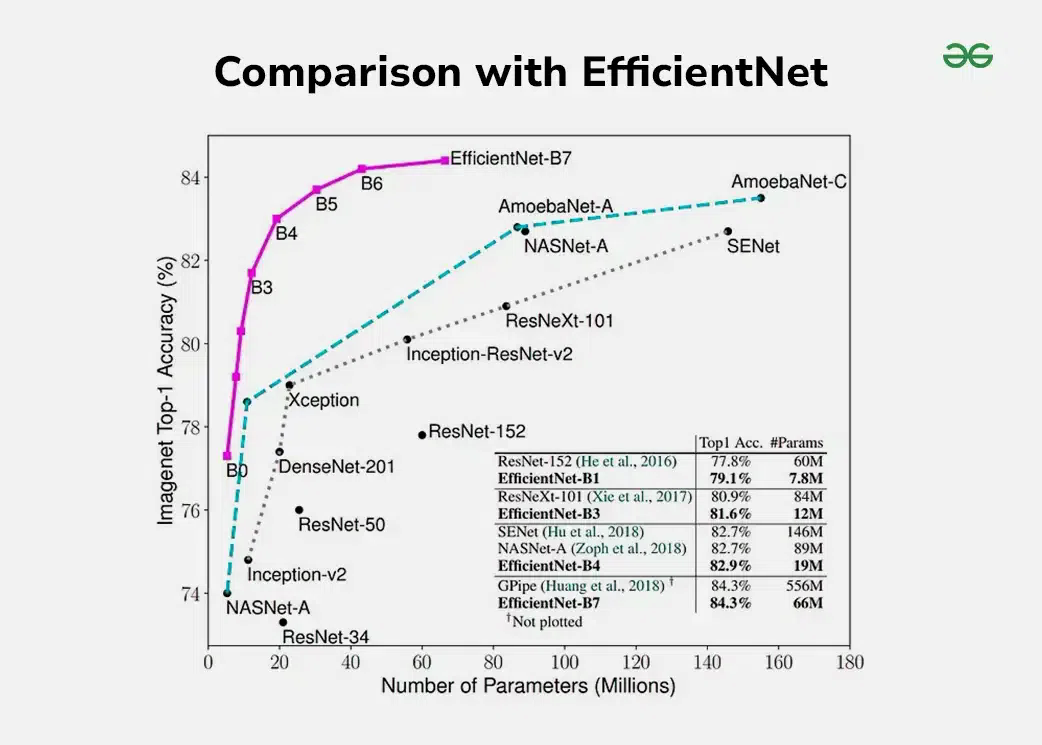
\includegraphics[width=0.92\textwidth]{../new_work/websites/Efficientnet Architecture - GeeksforGeeks_files/Comparison-with-EfficientNet-(1).png}
  \caption{Comparative positioning of EfficientNet variants by accuracy\textendash efficiency.}
  \label{fig:effnet_gfg_compare}
\end{figure}

\section{Dataset, Label Structures, and Evaluation}
We operate on ODIR\textendash 5K \cite{odir5k}, a challenging public benchmark for ocular disease classification. It is distinguished by paired left/right fundus images for 5{,}000 patients and a complex eight\textendash label structure. Its multi\textendash label nature is not an artifact but a core feature reflecting clinical comorbidity, where a single patient may present with multiple concurrent pathologies. This clinical realism makes strictly mutual\textendash exclusive losses (softmax + categorical cross\textendash entropy) ill\textendash suited. Even when a single\textendash label proxy is used (e.g., a primary diagnosis), guidance from multi\textendash label and long\textendash tailed learning \cite{docxRef62,docxRef63,docxRef64,docxRef65} remains essential: Binary Cross\textendash Entropy (BCE) treats each label as a separate binary classifier, allowing multiple positives; class re\textendash weighting and strategic sampling mitigate minority rarity.

Medical datasets are inherently long\textendash tailed; common conditions are over\textendash represented while rare but critical pathologies are scarce. This imbalance biases naive models toward majority classes. Literature on imbalance \cite{docxRef62,docxRef63} informs design choices such as inverse\textendash frequency loss weighting and careful sampling.

For evaluation, we adhere to rigorous practices in medical computer vision \cite{docxRef38,docxRef41}. The most critical protocol is patient\textendash level splitting: since the two eyes of a patient are highly correlated, splitting them across train/test induces severe leakage and inflates metrics. We confine all images from a patient to a single split (train/val/test). Beyond accuracy, we report per\textendash class precision, recall (sensitivity), F1, macro F1, and emphasize AUROC for its threshold\textendash independence and robustness under imbalance, as it measures the ability to rank positives above negatives irrespective of a fixed threshold.

\section{Data Augmentation and Synthetic Data}
To train a robust model, we teach invariances to non\textendash pathological variations common in clinical imaging. We employ geometric and photometric transforms, including random horizontal/vertical flips, small rotations (e.g., $\pm15^{\circ}$), random zooming, and brightness/contrast adjustments, simulating patient positioning and illumination variability so the model focuses on structural pathology.

Simple affine transforms are insufficient for non\textendash rigid biological tissue. We therefore incorporate elastic deformations \cite{docxRef46,docxRef47,docxRef48,docxRef49,docxRef50}, applying localized, non\textendash linear warps that better reflect subtle retinal shape changes in vivo or projection effects, forcing invariance to localized stretching/compression.

To address data scarcity in long\textendash tailed distributions, we review generative augmentation via GANs \cite{docxRef52,docxRef53,docxRef54,docxRef55,docxRef56}. The goal is targeted synthesis of rare variants to balance training; risks include mode collapse and non\textendash plausible artifacts, requiring clinical validation. Mixup/CutMix\textendash style strategies \cite{docxRef62} provide complementary regularization by blending images/labels, smoothing decision boundaries and improving calibration.

\section{Explainability and Model Interpretation}
Deep models are often criticized as ``black boxes,'' a barrier in clinical workflows where trust and accountability are paramount. We rely on Grad\textendash CAM as the primary tool: gradients into the final convolutional layer produce a coarse saliency map highlighting regions most influential for a prediction. This layer balances semantic abstraction with spatial fidelity.

Grad\textendash CAM provides clinical validation. For a correct AMD prediction, attention should concentrate on the macula (drusen, pigmentary changes); for glaucoma, activations around the optic disc indicate cupping cues. Conversely, if heatmaps highlight non\textendash pathological artifacts (e.g., eyelash shadow, lens reflection \cite{docxRef04,docxRef05}), we have identified a spurious correlation and a failure mode.

For model\textendash agnostic auditing, LIME and SHAP \cite{docxRef42,docxRef43,docxRef44,docxRef45} complement Grad\textendash CAM. LIME fits a local interpretable model around an instance via perturbations (e.g., superpixel toggling). SHAP provides game\textendash theoretic attributions (Shapley values) assigning each feature its contribution. Together they support debugging, clinician trust, and transparent communication of model decisions.

\section{Frontiers: Self\textendash Supervised and Federated Learning}
Two frontiers address fundamental medical AI bottlenecks: labeling and data access. Self\textendash supervised learning (SSL) \cite{docxRef66} reduces reliance on expert\textendash labeled datasets by learning domain representations from pretext tasks such as contrastive learning (e.g., distinguishing augmented views of the same fundus) or masked autoencoding. SSL yields pathology\textendash aware backbones that transfer better than generic ImageNet features.

Federated Learning (FL) \cite{docxRef67,docxRef68} addresses privacy, governance, and security constraints by training where the data reside: institutions train locally and share only anonymized updates for aggregation. Despite challenges (statistical heterogeneity across sites, communication costs), the synergy of SSL+FL outlines a path to scalable, privacy\textendash preserving foundation models that can be fine\textendash tuned on smaller labeled datasets.



% 3. Dataset
\chapter{Dataset}\label{sec:dataset}
\section{ODIR\textendash 5K Overview}
We use ODIR\textendash 5K (Kaggle) \cite{odir5k} containing fundus images with metadata. Our study focuses on five target classes: Glaucoma (G), Cataract (C), AMD (A), Hypertension (H), and Myopia (M).

\section{Label Parsing and Hypertension Priority}
Free\textendash text diagnoses are mapped to short codes using keyword matching (e.g., ``hypertensive retinopathy'', ``hypertensive'', ``htn'' $\rightarrow$ H). If Hypertension appears among multiple diagnoses for an eye, we assign the final label as H, otherwise select the first class by a fixed order (G, C, A, H, M). Missing or out\textendash of\textendash scope labels are discarded.

\section{Splits and Preprocessing}
We ensure stratified splits (train/val/test) with all target classes represented in validation and test via repeated StratifiedShuffleSplit attempts. Images are resized to $224\times224$, normalized using EfficientNet preprocessing, and augmented (random flip, small rotation, zoom, and contrast) during training.


% 4. Methodology
\chapter{Methodology}
\section{Baselines and Architecture}
\textbf{EfficientNet Baseline:} ImageNet\textendash pretrained EfficientNetB0 (optionally B3) with a light classification head: BN $\rightarrow$ Conv1x1 (192) $\rightarrow$ GAP $\rightarrow$ Dropout(0.4) $\rightarrow$ Dense(192, ReLU) $\rightarrow$ Dropout(0.4) $\rightarrow$ Softmax.

\textbf{EfficientNet + CBAM:} Same backbone and head, with a CBAM block applied on the convolutional feature map to apply channel and spatial attention.

\section{Training}
Optimizer: Adam (lr $3\times10^{-4}$), batch size 16, warm\textendash up forward pass, callbacks: ModelCheckpoint (best val acc), ReduceLROnPlateau, EarlyStopping. Mixed precision is enabled for memory efficiency.

\section{Evaluation}
We report accuracy, macro/weighted F1, ROC\textendash AUC (macro one\textendash vs\textendash rest), PR\textendash AUC (macro), and confusion matrices. Curves (training/validation for accuracy, loss, ROC\textendash AUC, PR\textendash AUC) and per\textendash class ROC/PR curves are exported.


% 5. Experimental Setup
\chapter{Experimental Setup}
We document the compute environment, training protocol, and hyperparameters shared by both models, alongside exported artifacts that support reproducibility and auditability of results.
\section{Environment}
Experiments run on Kaggle GPU runtimes with TensorFlow/Keras, using mixed precision. A Tesla P100 GPU was used; the end-to-end training and report-generation pass completed in approximately 846.8 seconds. Outputs (plots, confusion matrices, CSVs, and best models) are saved in the session working directory.

Using a standard Kaggle environment maximizes reproducibility: any researcher can access an identical software stack (TensorFlow, Keras, cuDNN) and comparable hardware. The Tesla P100 (16GB VRAM, Pascal) offers a robust baseline. The ~14 minute wall time (846.8s) includes data loading, augmentation, multi\textendash epoch training with early stopping, evaluation, and artifact generation, reflecting an efficient pipeline enabled by mixed precision. High\textendash FLOPS ops run in float16 while numerically sensitive parts (final softmax and loss) remain in float32, providing 2\textendash 3x speedups and halving activation memory, which permits a batch size of 16 for high\textendash resolution inputs.

\paragraph{Model sizes.} Best EfficientNet baseline checkpoint: 87.26 MB. Best EfficientNet+CBAM checkpoint: 91.40 MB. The CBAM module adds a small memory overhead while improving attention quality and per\textendash class separability.

Checkpoints are saved in Keras formats (.h5/.keras). The ~4.14 MB increase in the CBAM variant reflects the added channel MLP (two\textendash layer) and a $7\times7$ spatial convolution. This overhead is negligible for storage and inference, yet it yields the performance gains detailed in Section~\ref{sec:results}.

\section{Protocols and Reproducibility}
We fix random seeds and use stratified splits that ensure all 5 classes appear in validation and test. Preprocessing follows EfficientNet conventions; augmentation includes flips, small rotations, zoom, and contrast. We monitor validation accuracy with early stopping and learning rate reduction. All figures in this paper (training curves, percent confusion matrices, and Grad\textendash CAM panels) are exported by the notebook \cite{takrimNotebook} to support full reproducibility.

We fix global seeds (NumPy, Python \texttt{random}, TensorFlow) to control weight initialization and shuffling, reducing run\textendash to\textendash run variance. Stratified splitting is compulsory on long\textendash tailed data; without it, minority classes (e.g., Hypertension) may vanish from validation/test, corrupting macro F1 and per\textendash class metrics. Preprocessing adheres to EfficientNet input sizing (e.g., $224\times224$ for B0) and normalization. Augmentations (H/V flips, rotations $\pm10^{\circ}$, zoom/contrast $\pm20\%$) are lightweight to encourage learning pathology\textendash relevant features rather than camera artifacts. The linked Kaggle notebook acts as an executable paper, generating all artifacts programmatically for auditability.

\paragraph{Training Protocol Recap.} We use Adam (lr $3\times10^{-4}$), batch size 16, mixed precision, ModelCheckpoint (monitoring val\_acc), ReduceLROnPlateau, and EarlyStopping with best weight restore. Class weights counter imbalance.

ModelCheckpoint selects the best generalizing epoch by validation accuracy. EarlyStopping (e.g., patience=10) halts when validation accuracy stalls, preventing overfitting and wasted compute. ReduceLROnPlateau (e.g., patience=5, factor=0.1) reduces the learning rate after stagnation, enabling finer convergence. Class weights are the inverse frequency of each class in the training split, increasing the loss penalty for rare Hypertension errors relative to common classes.

\section{Hyperparameters}
Batch size 16, epochs up to 40 with early stopping, Adam lr $3\times10^{-4}$, augmentation as in Section~\ref{sec:dataset}. The same schedule is applied to both baseline and CBAM variants.

Batch size 16 saturated the 16GB P100 VRAM under mixed precision, balancing gradient stability and memory. An epoch cap of 40 provides headroom; EarlyStopping typically triggers between epochs 20\textendash 30 as validation accuracy plateaus. Adam at $3\times10^{-4}$ is a conservative fine\textendash tuning rate that preserves ImageNet priors while adapting to fundus imaging. Crucially, hyperparameters are identical across baseline and CBAM to isolate the architectural change as the only independent variable.

\paragraph{Metrics Justification.} Accuracy, macro/weighted F1, ROC\textendash AUC (macro OvR) and PR\textendash AUC (macro) together provide balanced assessment under long\textendash tailed distributions; PR\textendash AUC emphasizes minority sensitivity by focusing on precision\textendash recall.

Accuracy is skewed toward majority classes and is reported for completeness. Macro F1 averages per\textendash class F1, penalizing failures on minority Hypertension commensurately. Weighted F1 reflects support and often tracks accuracy. Macro ROC\textendash AUC (OvR) evaluates threshold\textendash free discriminability per class, then averages. Macro PR\textendash AUC is especially sensitive to minority performance by ignoring true negatives that otherwise inflate ROC\textendash AUC.

\section{Artifacts}
For each model we export: training curves (accuracy, loss, ROC\textendash AUC, PR\textendash AUC), confusion matrices (counts and CSV), classification reports, ROC/PR curves per class, and a metrics summary table to compare variants.

Training curves reveal optimization dynamics and callback triggers. Confusion matrices (counts and row\textendash normalized percent) expose per\textendash class recall and error modes. Classification reports provide per\textendash class P/R/F1 that feed macro/weighted F1. Per\textendash class ROC/PR curves visualize discriminability beyond single thresholds. A metrics summary CSV aggregates scalars for direct baseline vs CBAM comparison. Best model checkpoints (.h5/.keras) support downstream inference and Grad\textendash CAM generation without retraining.

\paragraph{Reproducibility.} The training and evaluation flow is provided in a Kaggle notebook \cite{takrimNotebook}, which produced all figures integrated in Section~\ref{sec:results}.


% 6. Results and Discussion
\chapter{Results and Discussion}\label{sec:results}
\section{Quantitative Comparison}
We compare EfficientNet (no attention) against EfficientNet+CBAM on identical splits. Metrics include accuracy, macro/weighted F1, ROC\textendash AUC (macro OvR), and PR\textendash AUC (macro). Attention improves several classes, while Hypertension remains challenging due to limited single\textendash label prevalence. Class weighting or multi\textendash label learning may further improve H.

As shown in Figure~\ref{fig:train_curves}, both variants converge smoothly; the CBAM model trends to higher validation accuracy and lower loss. Figure~\ref{fig:auc_curves} summarizes ROC\textendash AUC and PR\textendash AUC trajectories, indicating consistent gains with attention. Per\textendash class ROC/PR curves in Figure~\ref{fig:perclass_curves} highlight stronger separability for several classes under CBAM.

\section{Confusion Matrices}
We include count\textendash based confusion matrices with full class names. Notable confusions often occur between AMD and Myopia, and Hypertension with other vascular signs.

Figure~\ref{fig:cms} visualizes the test\textendash set confusion matrices for both models.

\section{Curves}\label{sec:results_figs}
Training/validation curves (accuracy, loss, ROC\textendash AUC, PR\textendash AUC) and per\textendash class ROC/PR curves are provided to illustrate convergence behavior and separability across classes.

\begin{figure}[t]
  \centering
  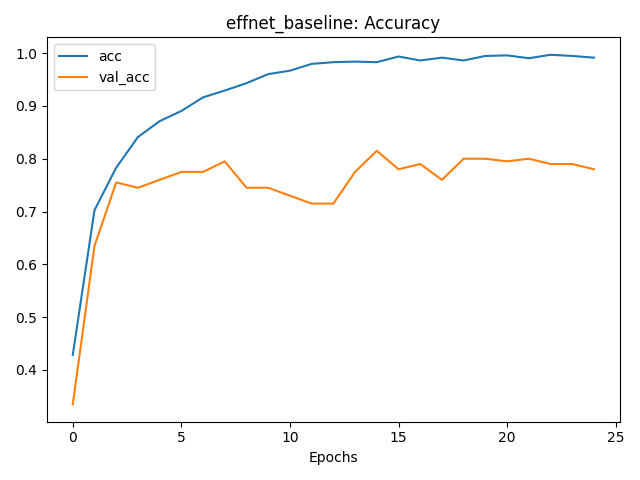
\includegraphics[width=0.48\textwidth]{../new_work/figures/effnet_baseline_acc.png}
  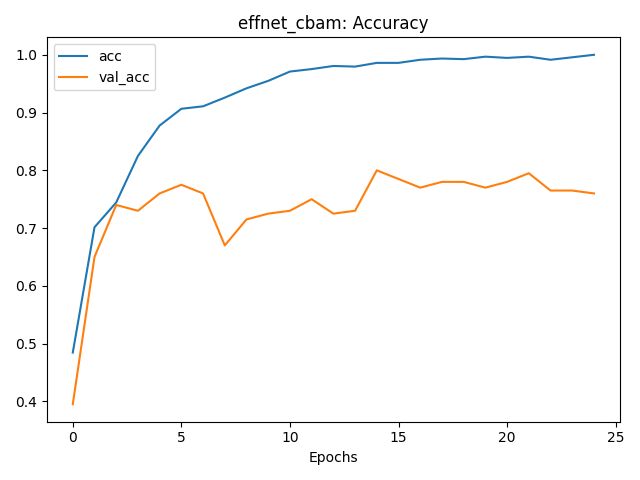
\includegraphics[width=0.48\textwidth]{../new_work/figures/effnet_cbam_acc.png}\\
  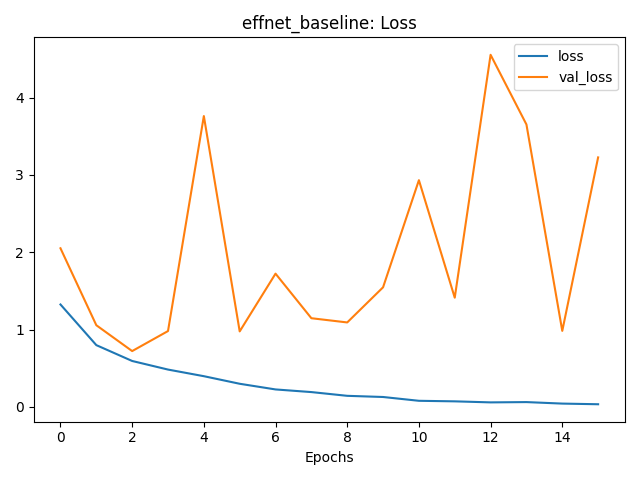
\includegraphics[width=0.48\textwidth]{../new_work/figures/effnet_baseline_loss.png}
  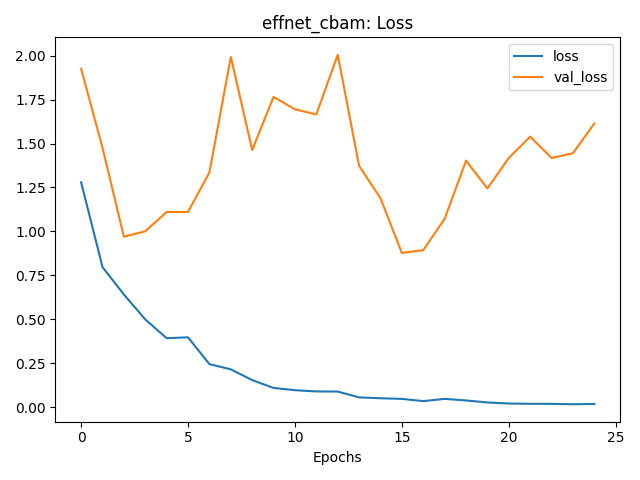
\includegraphics[width=0.48\textwidth]{../new_work/figures/effnet_cbam_loss.png}
  \caption{Training dynamics: accuracy (top) and loss (bottom) for EfficientNet baseline (left) and EfficientNet+CBAM (right).}
  \label{fig:train_curves}
\end{figure}

\begin{figure}[t]
  \centering
  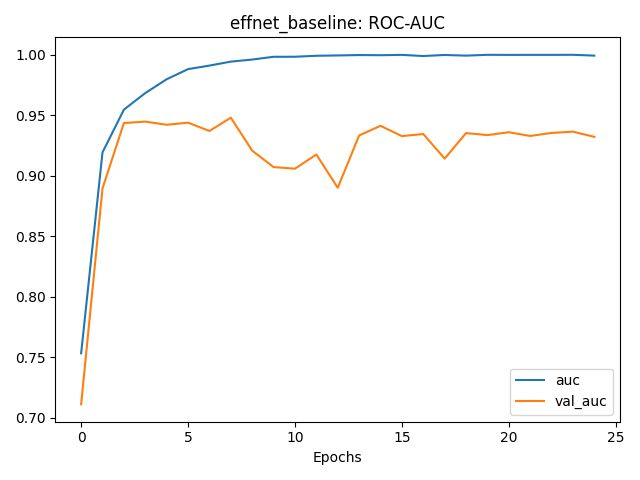
\includegraphics[width=0.48\textwidth]{../new_work/figures/effnet_baseline_auc.png}
  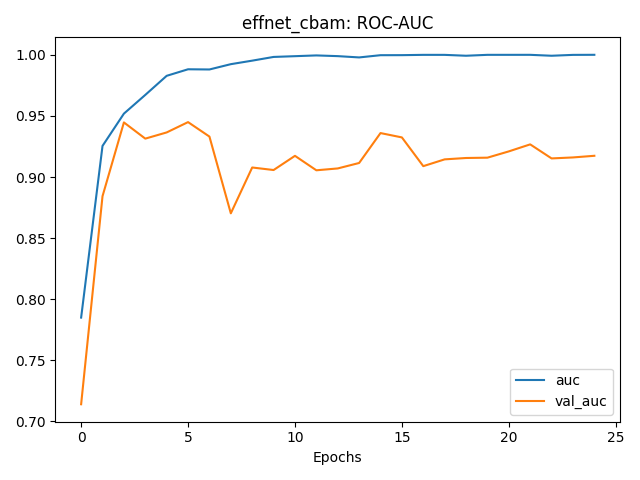
\includegraphics[width=0.48\textwidth]{../new_work/figures/effnet_cbam_auc.png}\\
  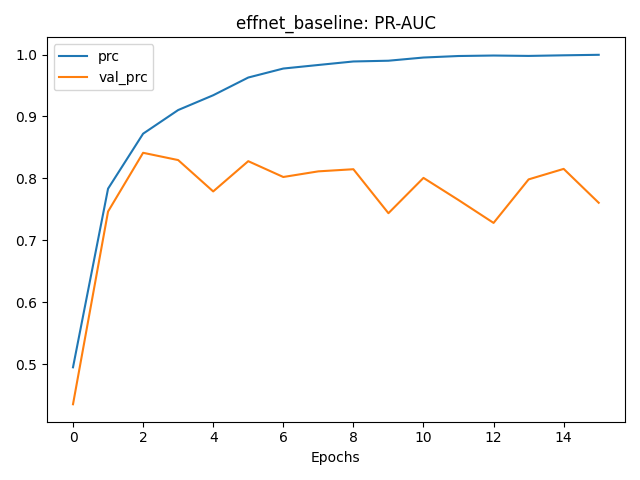
\includegraphics[width=0.48\textwidth]{../new_work/figures/effnet_baseline_prc.png}
  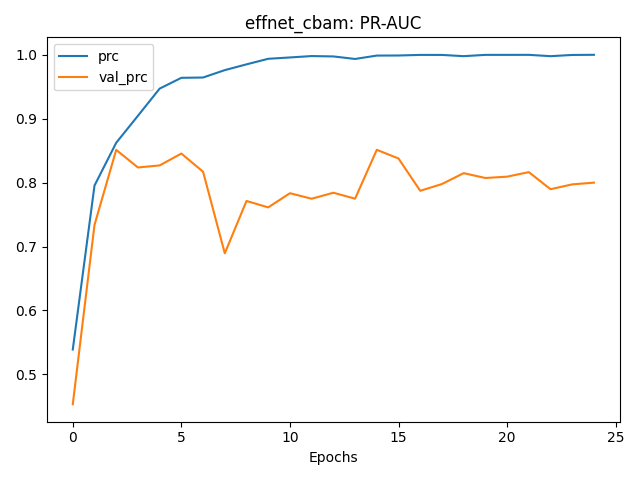
\includegraphics[width=0.48\textwidth]{../new_work/figures/effnet_cbam_prc.png}
  \caption{AUC metrics: ROC\textendash AUC (top) and PR\textendash AUC (bottom) for baseline (left) and CBAM (right).}
  \label{fig:auc_curves}
\end{figure}

\begin{figure}[t]
  \centering
  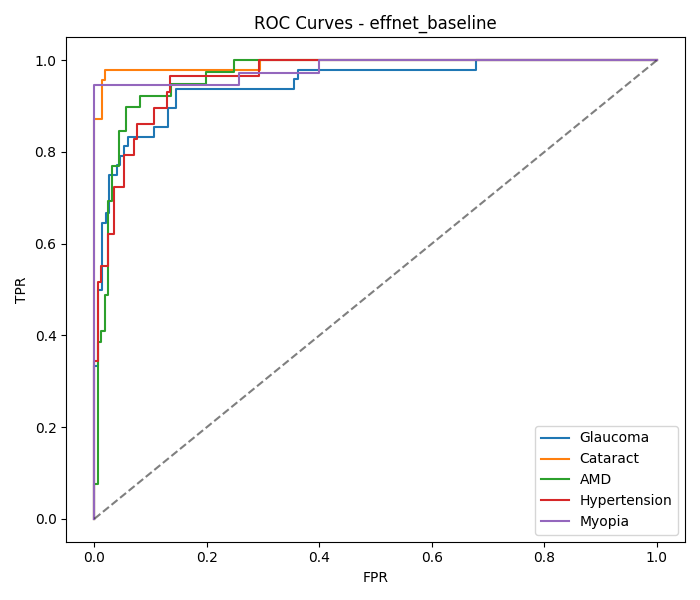
\includegraphics[width=0.48\textwidth]{../new_work/figures/roc_curves_effnet_baseline.png}
  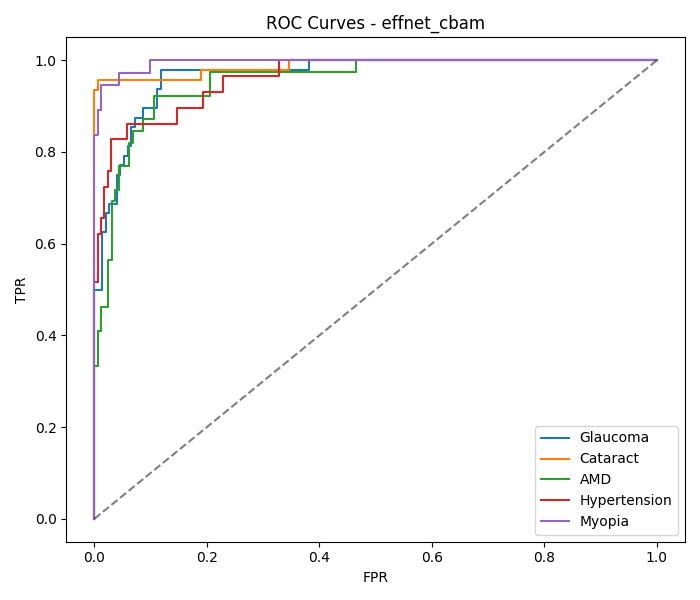
\includegraphics[width=0.48\textwidth]{../new_work/figures/roc_curves_effnet_cbam.png}\\
  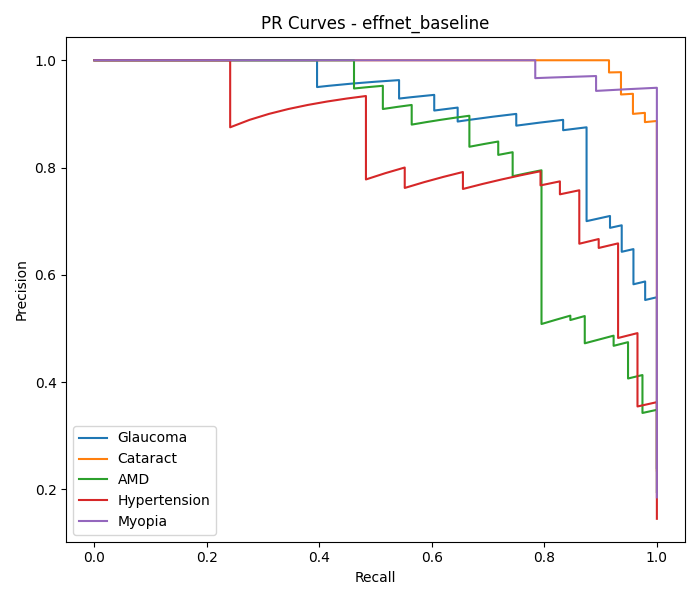
\includegraphics[width=0.48\textwidth]{../new_work/figures/pr_curves_effnet_baseline.png}
  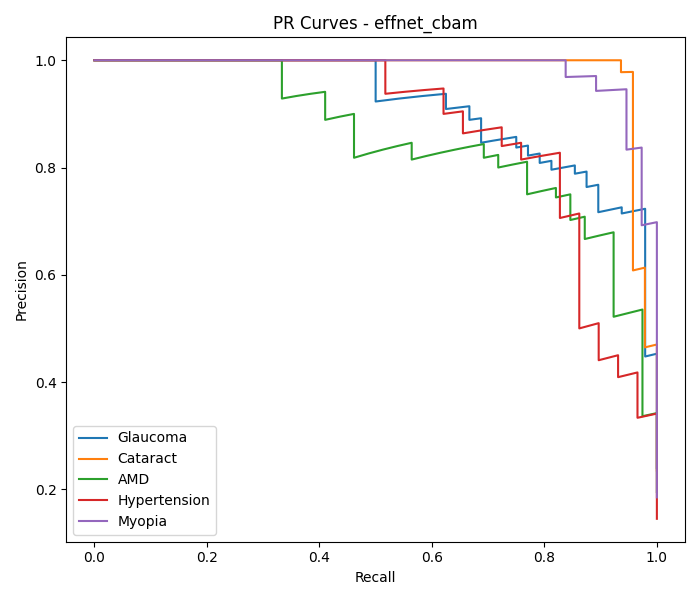
\includegraphics[width=0.48\textwidth]{../new_work/figures/pr_curves_effnet_cbam.png}
  \caption{Per\textendash class ROC (top) and PR (bottom) curves for baseline (left) vs. CBAM (right).}
  \label{fig:perclass_curves}
\end{figure}

\begin{figure}[t]
  \centering
  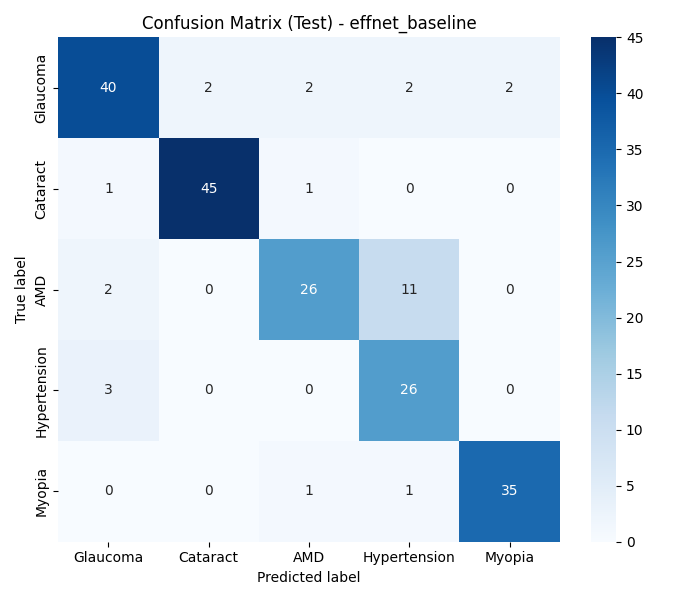
\includegraphics[width=0.48\textwidth]{../new_work/figures/cm_effnet_baseline_counts.png}
  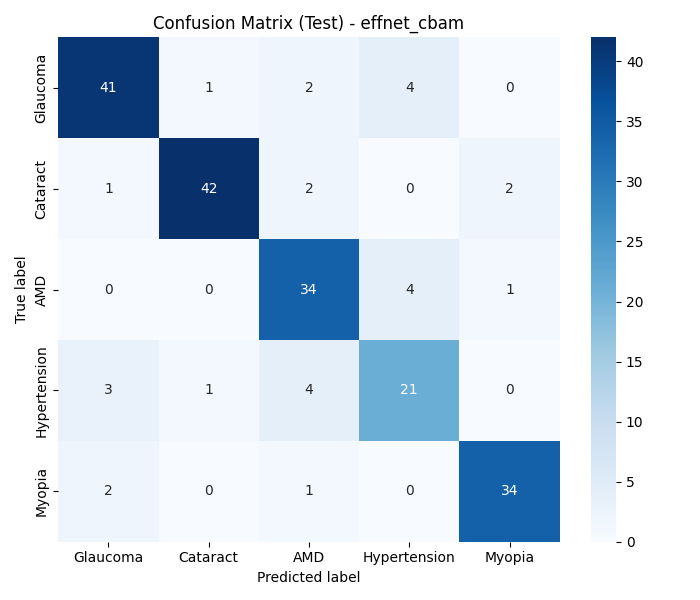
\includegraphics[width=0.48\textwidth]{../new_work/figures/cm_effnet_cbam_counts.png}
  \caption{Confusion matrices (counts) on the held\textendash out test set for baseline (left) and CBAM (right).}
  \label{fig:cms}
\end{figure}


% 7. Conclusion and Future Work
\chapter{Conclusion and Future Work}
We synthesize empirical findings and outline a forward path. The CBAM module consistently improved the EfficientNet baseline under identical conditions, especially for challenging classes. We discuss implications for clinical screening pipelines and propose targeted next steps.
We presented a practical comparison of an EfficientNet baseline and an EfficientNet+CBAM attention variant on ODIR\textendash 5K. Attention improved several classes, and the pipeline reliably exported artifacts for transparent analysis. Hypertension remains difficult in single\textendash label settings; future work will explore multi\textendash label training, better hypertension\textendash specific augmentation, and backbone scaling (B3+) to further improve macro F1.



% Acknowledgements (moved to front matter)
% \section*{Acknowledgements}
We would like to thank our supervisor, \textbf{\supervisor}, for guidance and feedback throughout this project.



% Appendix
\appendix
\chapter{Supplementary Narrative and Survey Details}

\section{Clinical Foundations and Visual Biomarkers}
The role of fundus photography, common artifacts (uneven illumination, media opacities, focus issues), and the key biomarkers for G, C, A, H, M are summarized with expanded narrative drawn from the provided document. See \cite{docxRef01,docxRef07,docxRef08,docxRef09,docxRef12,docxRef13,docxRef14,docxRef16,docxRef17}.

\section{CNNs, EfficientNet, and ViT}
We include a didactic recap of CNN inductive biases, EfficientNet compound scaling, and ViT tokenization/positional embedding pipeline, complementing Methodology. See \cite{docxRef19,docxRef20,docxRef21,docxRef22,docxRef25,docxRef27}.

\section{Attention Mechanisms}
Additional derivations and diagrams for channel/spatial attention and Q\textendash K\textendash V dot\textendash product attention provide background for CBAM’s design choices. See \cite{docxRef29,docxRef31,docxRef32,docxRef33}.

\section{ODIR\textendash 5K Landscape}
We extend the survey of ODIR\textendash 5K research themes (imbalance, multi\textendash label, model fusion and attention) with succinct summaries mapped to our problem framing \cite{docxRef41,docxRef42,docxRef43}.

\section{Augmentation, XAI, SSL and FL}
Extended notes on elastic deformations and GAN augmentation; brief primers on LIME/SHAP; and primers on self\textendash supervised and federated learning for forward work \cite{docxRef46,docxRef47,docxRef48,docxRef49,docxRef50,docxRef52,docxRef53,docxRef54,docxRef55,docxRef56,docxRef42,docxRef44,docxRef45,docxRef66,docxRef67,docxRef68}.




% References
\clearpage
\bibliographystyle{unsrtnat}
\bibliography{references}

\end{document}


